\documentclass{report}
\usepackage{setspace} % Setting line spacing
\usepackage{ulem} % Underline
\usepackage{caption} % Captioning figures
\usepackage{subcaption} % Subfigures
\usepackage{geometry} % Page layout
\usepackage{multicol} % Columned pages
\usepackage{array,etoolbox}
\usepackage{fancyhdr}
\usepackage{enumitem}
\usepackage[toc,page]{appendix}
\setlist{noitemsep}

% Page layout (margins, size, line spacing)
\geometry{letterpaper, left=1in, right=1in, bottom=1in, top=1in}
\setstretch{1.15}

% Headers
\pagestyle{fancy}
\lhead{PeaPod - Solution Overview}
\rhead{UTAG}

% Metric counter, referencing commands
\newcounter{metricnumber}
\setcounter{metricnumber}{1}
\newcommand{\metricrow}{M\arabic{metricnumber}}
\newcommand{\mlabel}[1]{\addtocounter{metricnumber}{-1}\refstepcounter{metricnumber}\label{#1}\addtocounter{metricnumber}{1}}
\newcommand{\mref}[1]{M\ref{#1}}

\begin{document}

\begin{titlepage}
    \begin{center}
        \vspace*{1.2cm}

        \textbf{\large{PeaPod - Solution Overview}}

        \vspace{0.5cm}

        Outlining a Design Proposal to the PeaPod Requirements

        \vfill \small{

            Jayden Lefebvre - Lead Engineer, UTAG Founder\\ECE 2T4 - University of Toronto - Toronto, ON, Canada\\Primary Contact: jayden.lefebvre@mail.utoronto.ca\\
            \vspace{.5cm}
            Nathan Chareunsouk - Industrial Designer\\Toronto, ON, Canada\\\vspace{.5cm}
            Navin Vanderwert - Design Engineer\\EngSci 2T4, University of Toronto - Toronto, ON, Canada\\\vspace{.5cm}
            Jonas Marshall - Electronics Engineer\\Computer Engineering 2024 at Queen's University - Kingston, ON, Canada

        }

        \vspace{2cm}

        Revision 0.6\\
        University of Toronto Agritech\\
        July 19th, 2021

    \end{center}
\end{titlepage}

\thispagestyle{plain}

\tableofcontents
\newpage

\section{Introduction}
\label{sec:intro}

\subsection{Purpose \& Design Process}
\label{sec:purpose}

The purpose of this document is to outline a design proposed to meet the PeaPod Requirements.

It accomplishes this via the following process:

\begin{figure}[h]
    \centering
    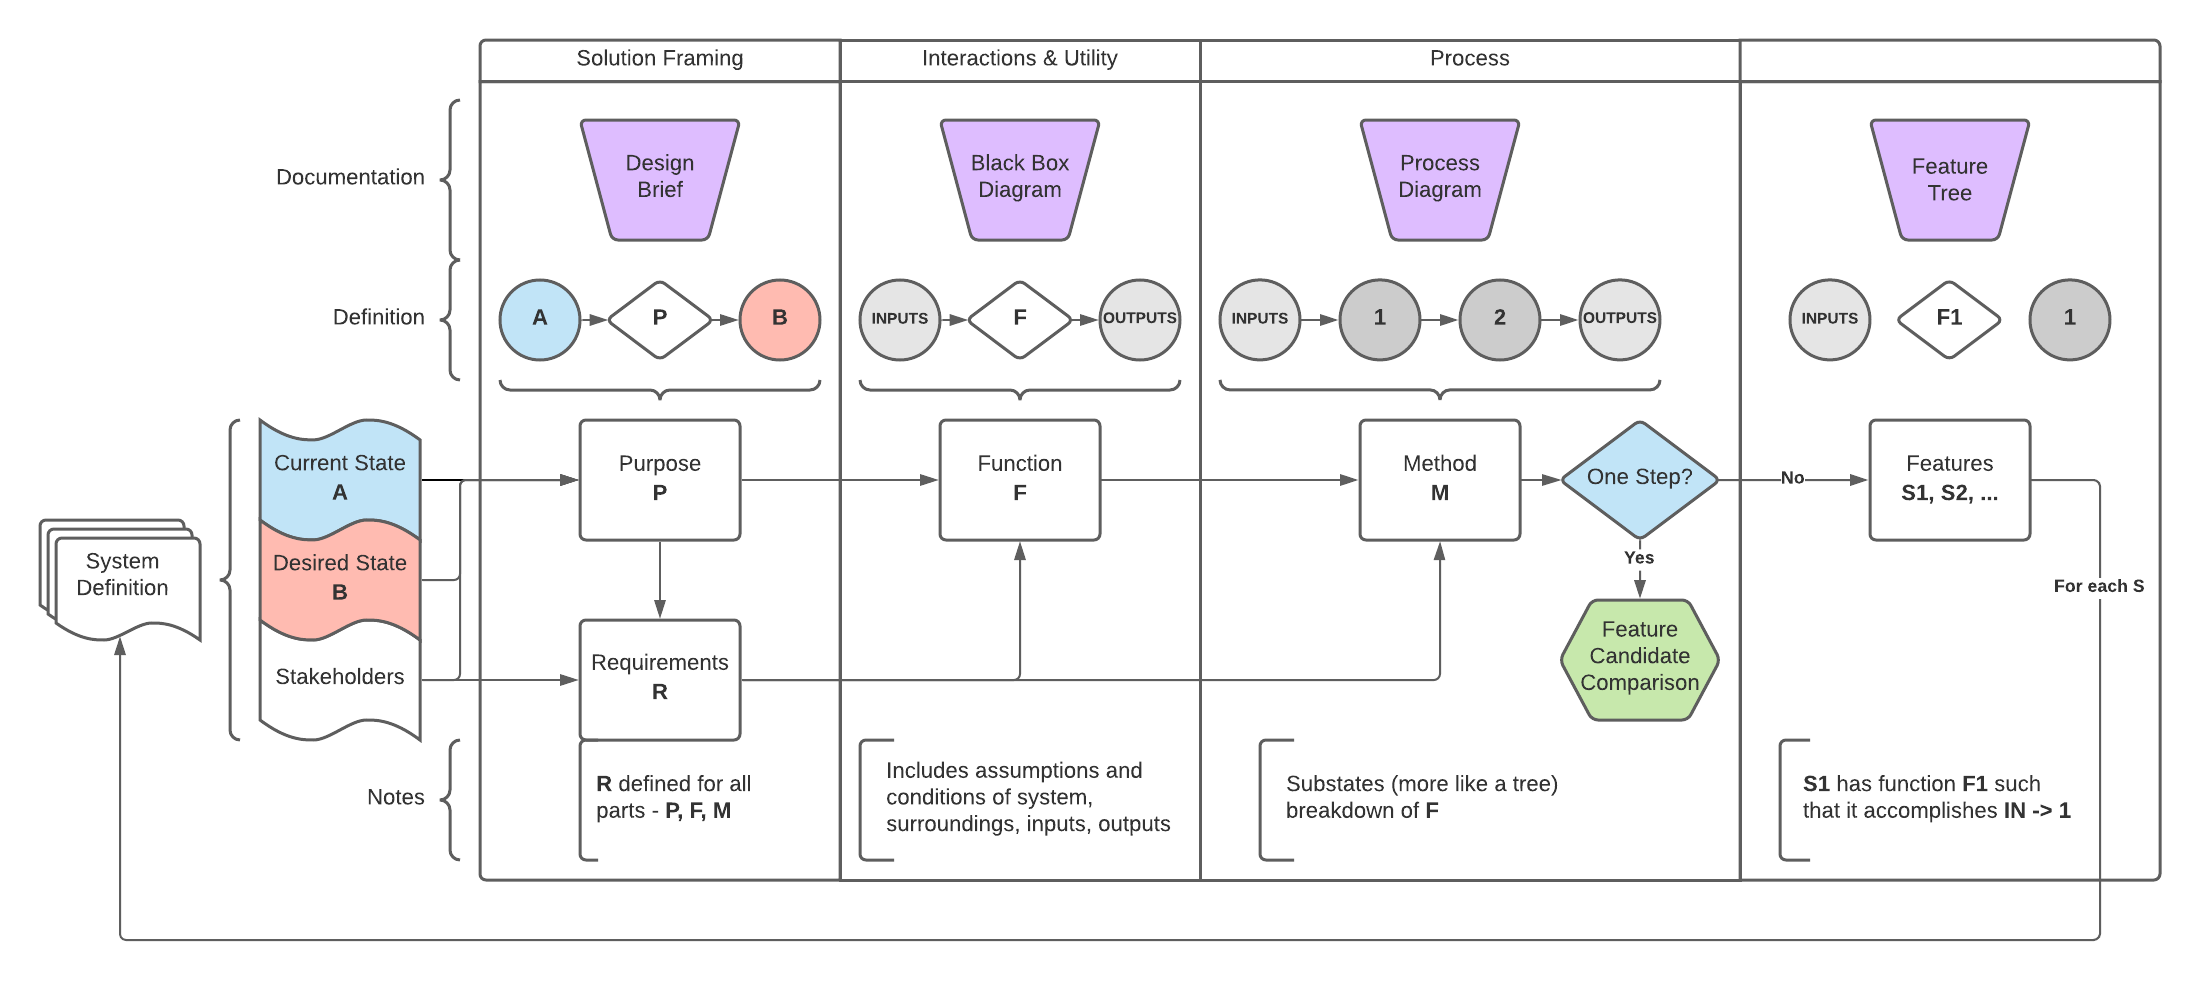
\includegraphics[width=16.5cm]{images/designprocess.png}
    \hfill
    \caption{Engineering design process.}
\end{figure}

\newpage

\section{Design}

\textbf{Purpose}: The purpose of the design is derived from the opportunity statement:

PeaPod is "an \uline{automated} and \uline{isolated} \uline{aeroponic} crop growth system, able to generate any \uline{growth environment} from a combination of independent \uline{environment parameters}, with both environment and crop growth \uline{data collection} for \uline{optimization}".

The primary function of the overall design is derived from both the overall purpose as well as the system inputs and outputs as defined by the DSFC Applicant Guide \cite{applicantguide}.

\textbf{Function}:

\begin{figure}[h]
    \centering
    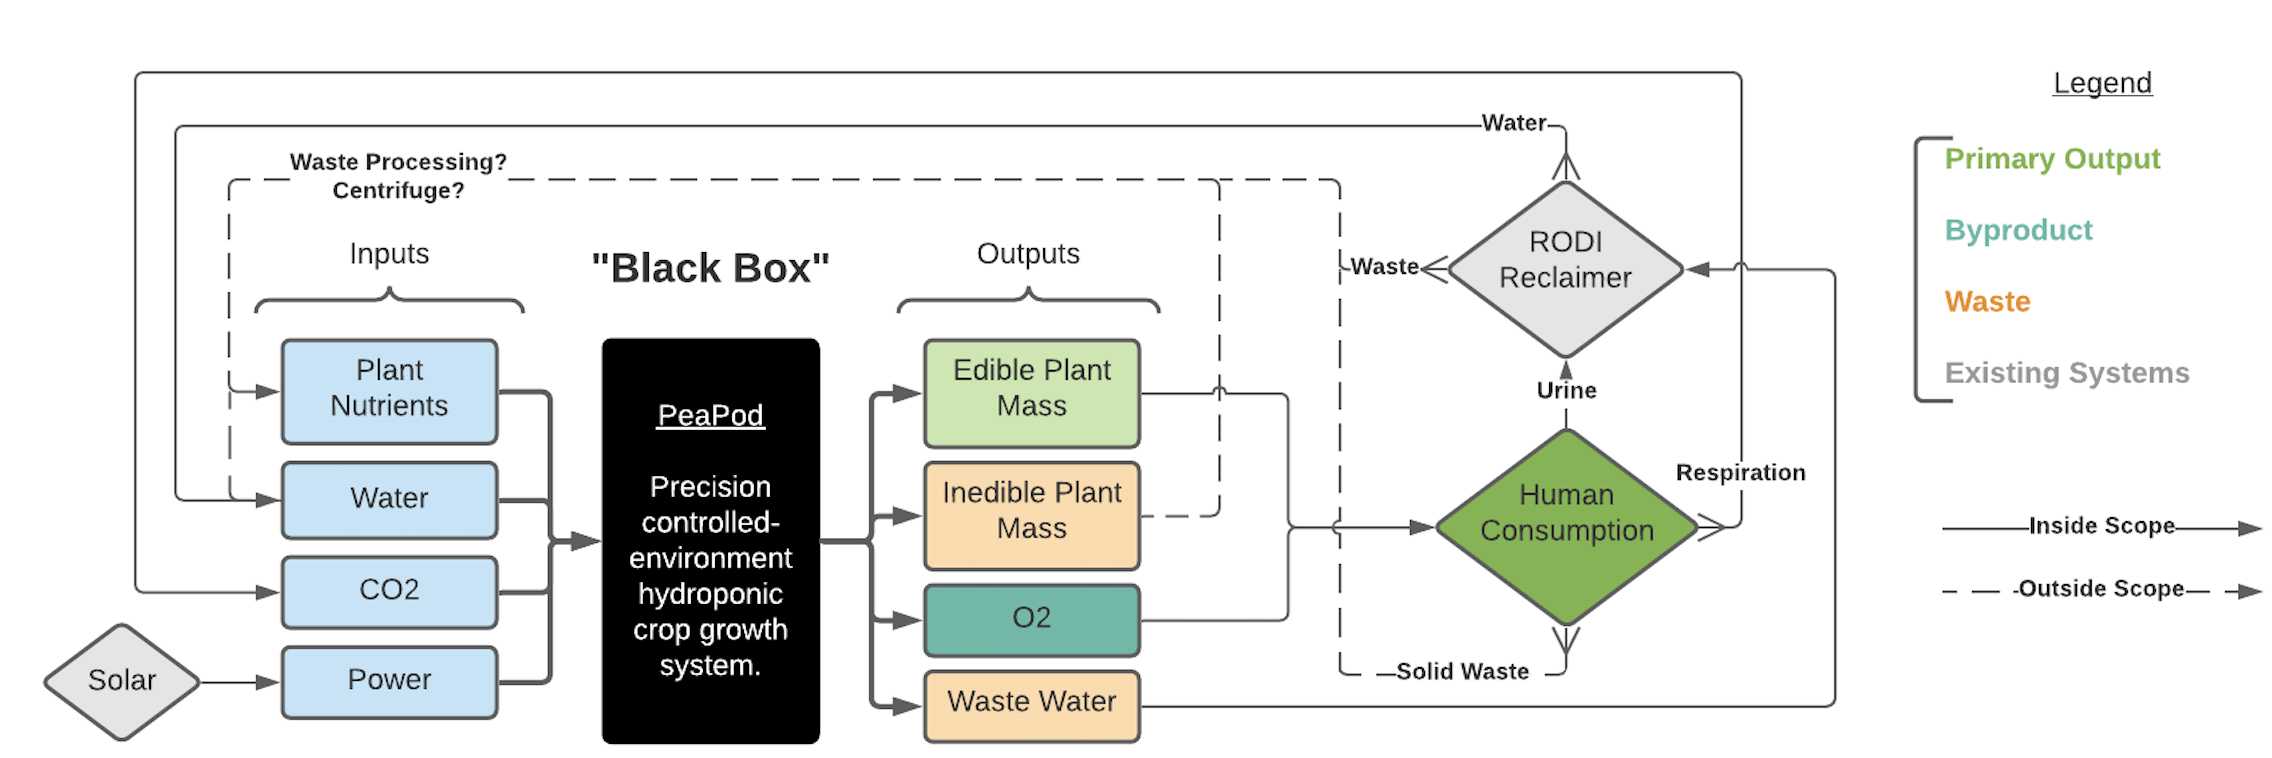
\includegraphics[width=15cm]{images/blackbox.png}
    \hfill
    \caption{"Black box" function diagram of PeaPod.}
\end{figure}

\textbf{Method \& Features}: 

\begin{figure}[h]
    \centering
    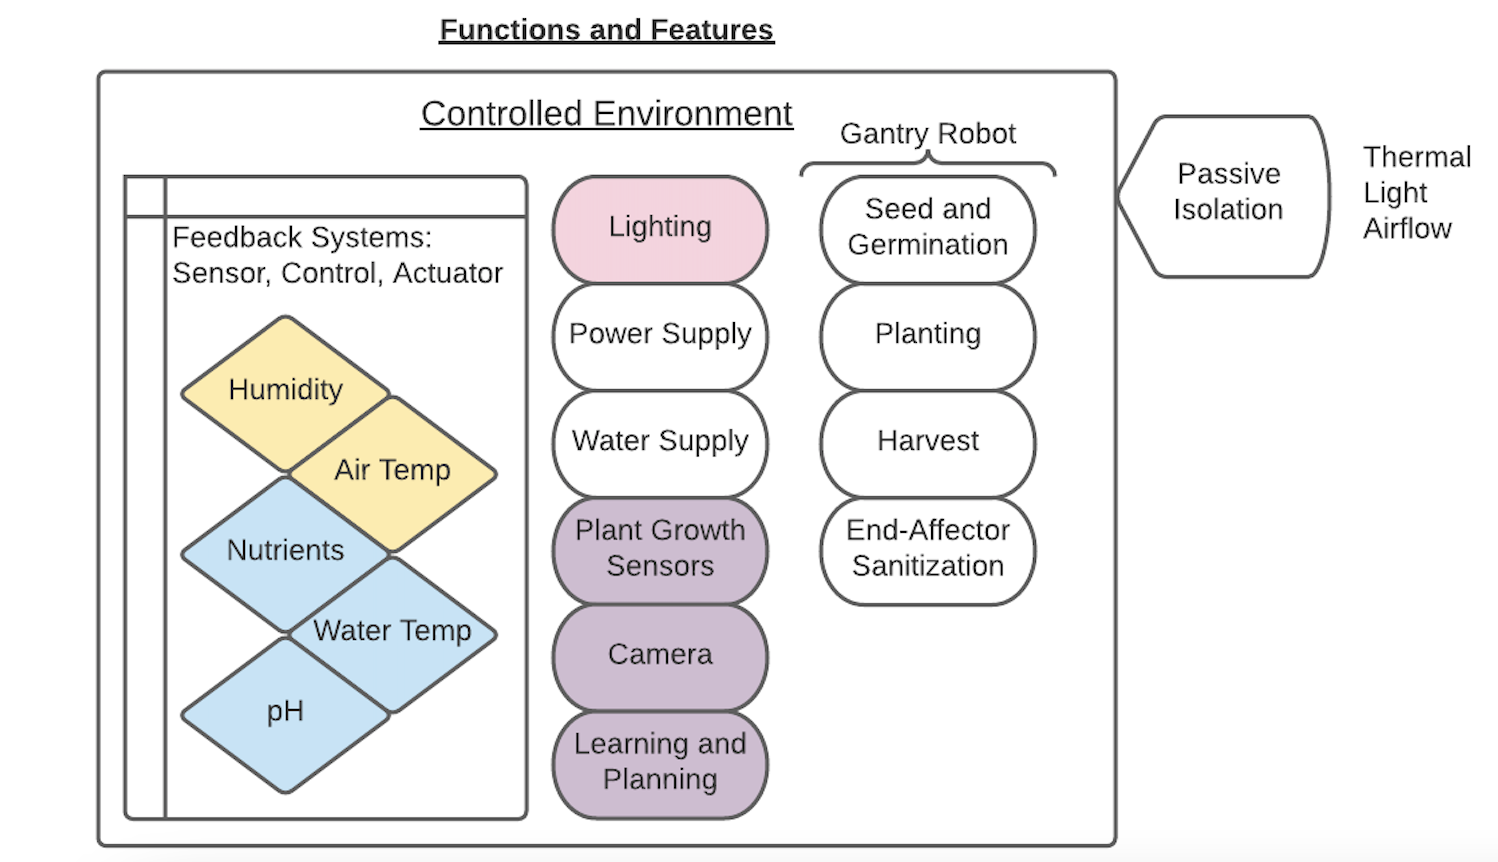
\includegraphics[width=12cm]{images/features.png}
    \hfill
    \caption{Features and feature types of PeaPod.}
\end{figure}

\newpage

\subsection{Automation}
\label{sec:automation}

\textbf{Purpose}: Performing growth-, maintenance-, and data-related tasks autonomously on the basis of both schedule and necessity to reduce crew maintenance time. Maintains the homogeneity of the internal environment.

\textbf{Function}:
\begin{itemize}
    \item \textbf{Inputs}: Environment sensor reading signals, program
    \item \textbf{Outputs}: Actuator control signals, crew messaging
\end{itemize}

\textbf{Method}:
\begin{enumerate}
    \item \textit{Setup}:
    \begin{enumerate}
        \item Power is connected and system is booted;
        \item Program is inputted by user;
    \end{enumerate}
    \item \textit{Testing}:
    \begin{itemize}
        \item Power-on Self-Test (POST) passes;
        \item Systems enact program as intended;
    \end{itemize}
    \item \textit{Process}:
    \begin{enumerate}
        \item Checks operating preconditions (self POST and per-subsystem);
        \item \textbf{Environment Control Loop}:
        \begin{enumerate}
            \item Receives and stores data about current environment state;
            \item Compares current state to desired state, develops a "plan" to reach desired state;
            \item Controls subsystem operations in order to enact the plan;
        \end{enumerate}
        \item Notifies user on maintenance requirement (i.e. non-automated input/output management, refills, repairs, etc.);
    \end{enumerate}
    \item \textit{Shutdown} (either manual or end-of-program/EOP):
    \begin{enumerate}
        \item Stop subsystem operations;
        \item \textit{If EOP}: Notify user;
    \end{enumerate}
\end{enumerate}

\textbf{Features}:
\begin{itemize}
    \item \textit{Computer System}: Manages \textbf{all} data collection, storage, analysis, and transmission/receiving, as well as planning and actuator control. Includes internal clock (for program, notification), network connection (for data transmission, notification), and storage (for data). 
\newpage
    \item \textit{Camera}: Multiple angles. For live feed transmission to users (local and remote), as well as plant health and yield metric collection via \textbf{computer vision analysis}. Metrics include:
    \begin{itemize}
        \item Leaf health indicators (i.e. leaf tip burn, leaf curl, chlorosis);
        \item Leaf count, size distribution;
        \item Leaf density;
        \item Canopy dimensions/surface area;
        \item Plant height;
        \item Fruit/harvest body size, ripeness;
        \item etc.
    \end{itemize}
    \item \textit{Environment Sensors}: Record the environment's current state. Covers each environment control loop (see \ref{sec:environment} \textbf{outputs}), as well as CO${}_2$ ppm.
    \item \textit{Diagnostic Systems}: Include informative sensors tracking system input availability, etc. as well as notification triggers.
    \item \textit{Program}: Set of action (e.g. lights on) and control target (e.g. hold air temperature at 22°C) \textbf{time-series} instructions;
    \item \textit{Actuators}: Induce a change. Covers each environment control (see \ref{sec:environment}, \ref{sec:lighting} \textbf{inputs});
\end{itemize}

\textbf{Justification}: 
\begin{itemize}
    \item \textbf{Purpose}: Increased accuracy/precision over human interference, minimize human hours spent. Enables control over all parameters simultaneously.
    \item \textbf{Method}: Environment data and plant metrics match $\vec E,\vec P$ respectively from the optimization routine (see Section \ref{sec:optimization}). Control loop model matches \textit{Sense-Plan-Act} model of robotics, and is well suited for controlled-environment agriculture.
\end{itemize}

\newpage

\subsection{Housing}
\label{sec:housing}

\textbf{Purpose}: \textit{Isolates} and \textit{insulates} growth environment from exterior environment (heat, light, humidity). Provides structural integrity and mounting points for other subsystems.

\textbf{Method}:
\begin{enumerate}
    \item \textit{Setup}:
    \begin{enumerate}
        \item Construct frame and install panels;
        \item Mount control module (w/ subsystems), connect inputs and internal subsystem connections;
        \item Install tray mounts, insert trays (w/ subsystems);
    \end{enumerate}
    \item \textit{Testing}:
    \begin{itemize}
        \item Frame construction is rigid, level, and sturdy;
        \item Panels are insulating against temperature changes;
    \end{itemize}
    \item \textit{Process}:
    \begin{enumerate}
        \item Panels insulate against heat gain/loss, are opaque, and contain light and heat via reflection;
        \item Shell construction is tight, thus sealing against moisture;
        \item Internal vertical mounting channels for systems, horizontal plane "trays";
        \item \textbf{Extension} (can be repeated):
        \begin{enumerate}
            \item Add a second housing;
            \item Remove dividing panel from both housings;
            \item Remove "shared" skeleton extrusions from second housing;
            \item Join the two housings to form one larger 2x1 housing;
            \item \textbf{Extension Modes} (may be combined in any way to suit application):
            \begin{itemize}
                \item \textit{Option 1} (Smaller Housings): Operate the combined housing off \textbf{one} control module.
                \item \textit{Option 2} (Larger Housings): Add a control module to account for additional air volume, plant count, power requirement, etc.. Operate in a \textbf{controller-follower topology}.
                \item \textit{Option 3} (Frame Connection Only): Leave the dividing panel, add a control module, and operate the two PeaPods \textbf{separately}.
            \end{itemize}
        \end{enumerate}
    \end{enumerate}
    \item \textit{Shutdown}:
    \begin{enumerate}
        \item Dismount all systems, remove trays;
        \item Disassemble housing;
    \end{enumerate}
\end{enumerate}

\newpage

\textbf{Features}:
\begin{itemize}
    \item \textit{Frame}: Cubic skeleton made of aluminum extrusion with standard mounting channels. "Edges" of cube.
    \item \textit{Panels}: Foam insulation panels with mylar internal coating. Panels slide into extrusion channels. "Faces" of cube.
    \item \textit{Trays}: Horizontal plane subframes mounted to internal vertical extrusion channels for ease of repositioning. Trays slide in/out on permanent mounts. All connections are \textit{quick-disconnect} (i.e. quick-connect tubing for grow tray, push connectors for lighting) for ease of removal. Trays include:
    \begin{itemize}
        \item \textit{Grow Trays}: Support plants (via grow cups), aeroponic nozzles, and aeroponics container (See \ref{sec:aeroponics}).
        \item \textit{Lighting Trays}: Support LED boards, driver board (See \ref{sec:lighting}).
    \end{itemize}
\end{itemize}

\textbf{Justification}: 
\begin{itemize}
    \item \textbf{Function}: Insulation increases thermal and light efficiency. Isolation increases safety against cross-contamination, pathogens, harmful substances.
    \item \textbf{Method}: Solid frame-and-panel construction is efficient for packing away, and is honestly just simple. Adaptable tray subframes make future feature development easier, and allows to modularly swap subsystems.
    \item \textbf{Features}: Aluminum extrusion is commonly used for frames, and has a high strength-weight ratio. Allows strong, repositionable mounting via channels. Foam insulation is highly insulating and opaque, and mylar ensures internal light reflection. Sliding directly into extrusion channels boosts "seal".
\end{itemize}

\newpage

\subsection{Aeroponics}
\label{sec:aeroponics}

\textbf{Purpose}: Delivers nutrients and pH-balanced, temperature-controlled water to the plant roots via a fine mist.

\textbf{Function}:
\begin{itemize}
    \item \textbf{Inputs}: Reverse osmosis water under positive pressure, pH up \& down solutions, concentrated nutrient solutions, pump control (on/off to relay for pump power), nozzle control (on/off to relay for solenoid power), pH and nutrient solution ratios as signals (stepper positions/valve open percent), thermoregulation power as signal (PWM to H-bridge polarity switch to MOSFET to Peltier), thermoregulation fan power
    \item \textbf{Outputs}: Mist (50 micron mean droplet diameter)
\end{itemize}

\textbf{Method}:
\begin{enumerate}
    \item \textit{Setup} (comes pre-assembled):
    \begin{enumerate}
        \item Hook up all inputs;
        \item Connect the quick-disconnect fitting;
        \item Fill nutrient, pH solution containers;
        \item Calibrate pressure, temperature sensors to atmospheric;
        \item Enable water input to prime system (if known pressure/temperature, calibrate sensors);
    \end{enumerate}
    \item \textit{Testing}:
    \begin{itemize}
        \item Temperature, pressure sensors communicate as expected;
        \item No leaks at any connections under a) source pressure, b) fully pressurized;
        \item Pump auto-shuts off near 80PSI;
        \item Tubing and all components withstand full pressurization;
        \item Solenoid is normally closed, withstands full pressurization, and opens when power is applied;
        \item Quick-disconnect operates as intended at full pressurization without leaks;
        \item Nozzles produce full-cone mist;
        \item Manual and servo-actuated valves operate as intended;
    \end{itemize}
    \item \textit{Process}:
    \begin{enumerate}
        \item Water is pressurized to constant 80PSI;
        \item Heat is added to or removed from the water (\ref{sec:automation}); % TODO: Add water temp to environment control?
        \item Temperature and pressure of the water is read (feeds back);
        \item Nutrient and pH (\ref{sec:nutrientsph}) solutions are mixed in-line at an adjustable ratio (\ref{sec:automation}); \footnote{I.e. add X mL of nutrient solution Y per mL water to achieve Z ppm, or add A mL of pH down solution per mL water to achieve a pH of B.}
        \item Flow to nozzle is controlled (on/off) (\ref{sec:automation});
        \item Nozzle turns pressurized water into mist;
    \end{enumerate}
\newpage
    \item \textit{Shutdown}:
    \begin{enumerate}
        \item Power down the pump and thermoregulation unit;
        \item Close the nutrient and pH solution valves;
        \item Close the source shutoff valve;
        \item Open the drain valve, and allow the system to depressurize and  drain completely;
        \item Power down the solenoid;
        \item Disconnect the quick-disconnect fitting;
        \item Disconnect the inputs;
    \end{enumerate}
\end{enumerate}

\textbf{Features} (in order of plumbing; source $\to$ nozzle):
\begin{itemize}
    \item \textit{Water Source}: Input for reverse-osmosis water.
    \item \textit{Manual Source Shutoff Valve}
    \item \textit{Diaphragm Pump}: Self-priming, auto-shutoff at 80psi. Power is controlled by external relay signal (\ref{sec:automation}).
    \item \textit{Inline Water Heater/Cooler}: Thermoelectric heater/cooler. Peltier tiles (H-bridge polarity control, PWM dimming), aluminum water block/heat sink combo, and fans.
    \item \textit{Accumulator Tank}: Uses an air bladder to create and stabilize pressure.
    \item \textit{Pressure Sensor}: Reports to computer (\ref{sec:automation}). Allows for shutoff of pump in case of emergency.
    \item \textit{Manual Drain Valve}: Ball valve. Allows the system to be depressurized and drained.
    \item \textit{Nutrient and pH Adjustment Solutions}: Section \ref{sec:nutrientsph}
    \item \textit{Adjustable-rate Siphon Injection Manifold}: Section \ref{sec:manifold}.
    \item \textit{Solenoid Valve}: Enables on-demand (\ref{sec:automation}) misting.
    \item \textit{Grow Tray Quick-Disconnect}: Connectors between aeroponics supply and nozzles that allow for quick disconnection with auto-shutoff so the trays may be removed.
    \item \textit{Nozzle}: Mounted to grow tray, pointed at plant roots. 80psi water through a 0.4-0.6mm orifice produces 5-50 micron water droplets. %TODO: Source??
\end{itemize}

\textbf{Justification}: 
\begin{itemize}
    \item \textbf{Purpose}: A high pressure aeroponics system eliminates water parameter feedback, and is 98\% more water efficient than traditional farming.
    \item \textbf{Function}: RO water has no dissolved nutrients and a neutral pH of 7.0. This enables easier and more reliable calculations. In addition, it has no particulate or minerals, minimizing the chances of nozzle clog.
    \item \textbf{Method}: System is medium-free, eliminating risk of pathogens developing within root zone. Using a nozzle ensures the nutrient solution is evenly distributed. Mean droplet size of 5-50 microns is optimal for plant growth. %TODO: Source?? also more detail here
\end{itemize}

\newpage

\subsubsection{Solution Nutrients and pH}
\label{sec:nutrientsph}

\textbf{Purpose}: Providing all necessary plant nutrients at the correct pH.

\textbf{Function}:
\begin{itemize}
    \item \textbf{Inputs}: Plant nutrients, pH up solution, pH down solution (all stored)
    \item \textbf{Outputs}: Plant nutrients, pH up solution, pH down solution (on-demand)
\end{itemize}

\textbf{Method}:
\begin{enumerate}
    \item \textit{Setup}:
    \begin{enumerate}
        \item Fill containers with nutrient, pH solutions;
        \item Install and connect fill level sensors;
        \item Install output tubes;
    \end{enumerate}
    \item \textit{Testing}:
    \begin{itemize}
        \item No container leaks;
        \item Fill level sensors operate as intended;
    \end{itemize}
    \item \textit{Process}:
    \begin{enumerate}
        \item Solutions are held in containers;
        \item Solutions are siphoned from containers on-demand;
        \item Fill level sensors notify user (\ref{sec:automation}) when empty;
    \end{enumerate}
    \item \textit{Shutdown}:
    \begin{enumerate}
        \item Empty containers;
        \item Disconnect fill level sensors and output tubes;
    \end{enumerate}
\end{enumerate}

\textbf{Features}:
\begin{itemize}
    \item \textit{Nutrient Solutions}: Aqueous. Highly concentrated. Selectable as part of the program (\ref{sec:automation})\footnote{Many different solutions can be combined (according to solubility laws, pH requirements, etc.).}, and may include any of:
    \begin{itemize}
        \item Bioavailable nonmetals (ammonia, ammonium, nitrates, nitrites, phosphates, sulfates, etc.)
        \item Bioavailable metals (potassium, etc.)
        \item Minerals (magnesium, calcium)
        \item Other trace elements
        \item Custom solutions (i.e. fungicides/algicides)
    \end{itemize} 
    \item \textit{pH Adjustment Solutions}\footnote{\textit{NOTE:} Ionic composition of pH solutions should be considered in the understanding of the spray (i.e. phosphic acid results in phosphate ions in spray)}: Aqueous. Highly concentrated. One for pH up (>8), one for pH down (<6).
    \item \textit{Solution Storage Containers}: Opaque, insulated, chemical-safe, refillable cartridges.
    \begin{itemize}
        \item \textit{Fill Level Sensors}: Depth sensors measure fill level of container.
    \end{itemize}
\end{itemize}

\textbf{Justification}: 
\begin{itemize}
    \item \textbf{Features}: Opaque and insulated cartridges prevent degradation of compounds over time via light or heat (respectively). Built-in level sensors allow for notification to refill.
\end{itemize}

\subsubsection{Solution Injection Manifold}
\label{sec:manifold}

\textbf{Purpose}: A manifold of parallel in-line injectors, allowing for adjustable mixing ratios for nutrient and pH solutions.

\textbf{Function}:
\begin{itemize}
    \item \textbf{Inputs}: Pressurized RO water, per-solution flow-ratio control signal (calculated from desired per-nutrient concentrations; \ref{sec:automation}), pH flow-ratio control signal (calculated from desired pH; \ref{sec:automation})
    \item \textbf{Outputs}: Pressurized mixed solution with set pH and nutrient concentrations
\end{itemize}

\textbf{Method}:
\begin{enumerate}
    \item \textit{Setup}:
    \begin{enumerate}
        \item Connect inlet lines to siphon inlets;
        \item Connect solution containers to inlet lines;
        \item Connect flow control servos to control module;
    \end{enumerate}
    \item \textit{Testing}:
    \begin{itemize}
        \item Flow control servos and valves operate as intended;
        \item Injection ratios are accurate;
        \item Check valves prevent backflow when solenoid is closed;
    \end{itemize}
    \item \textit{Process}:
    \begin{enumerate}
        \item Water splits into parallel injection "branches";
        \item Each branch injects solution at an adjustable (\ref{sec:automation}) ratio (flow:flow);
        \item Branches recombine;
    \end{enumerate}
    \item \textit{Shutdown}:
    \begin{enumerate}
        \item Disconnect inlet lines from siphons, containers;
        \item Disconnect flow control servos from control module;
    \end{enumerate}
\end{enumerate}

\textbf{Features}:
\begin{itemize}
    \item \textit{Venturi Siphons}: Venturi-based siphons for flow-ratio injection of solutions (one siphon per solution).
    \item \textit{Input, Output Manifold}: Manifolds for distribution of water to branches, and recombination of solution post-injection.
    \item \textit{Flow Control Valves}: Completely adjustable flow control, driven by servos.
    \item \textit{Check Valves}: Prevents backflow through siphon inlet when output solenoid is closed.
\end{itemize}

% TODO: Justification?

\newpage

\subsection{Environment Control}
\label{sec:environment}

\textbf{Purpose}: Subsystems responsible for generating the internal plant growth environment, providing control over all relevant environment parameters. Provides sensing and acting peripherals to the control module's automation system (\ref{sec:automation}).

\textbf{Function}:
\begin{itemize}
    \item \textbf{Inputs}: Power, water, environment control parameters (as signals)
    \item \textbf{Outputs}: Environment sensor values, controlled environment
\end{itemize}

\textbf{Method} (informed by \ref{sec:automation}):
\begin{enumerate}
    \item \textit{Setup}:
    \begin{enumerate}
        \item Connect power, water inputs;
        \item Connect all actuator input signals and sensor output signals to control module;
    \end{enumerate}
    \item \textit{Testing}:
    \begin{itemize}
        \item Each subsystem responds properly to automation (\ref{sec:automation}) control;
        \item Each control loop system sensor reports accurately;
    \end{itemize}
    \item \textit{Process}:
    \begin{enumerate}
        \item Sensor signals sent to automation (\ref{sec:automation});
        \item Actuator control signals received from automation (\ref{sec:automation});
        \item Actuators respond to control signals to control:
        \begin{itemize}
            \item Leaf zone air temperature\footnotemark[4];
            \item Leaf zone humidity\footnotemark[4];
            \item Root zone/aeroponics temperature\footnote{Control Loop (aka Feedback) System - includes sensor(s)};
            \item Air Composition (CO${}_2$/O${}_2$)\footnotemark[4];
            \item Lighting spectrum and intensity\footnote{Set System - no feedback sensors};
            \item Aeroponics delivery/"flow" rate\footnotemark[5];
            \item Aeroponics solution per-nutrient concentrations\footnotemark[5];
            \item Aeroponics solution pH\footnotemark[5];
        \end{itemize}
    \end{enumerate}
    \item \textit{Shutdown}:
    \begin{enumerate}
        \item Disconnect inputs;
        \item Disconnect control module connections;
    \end{enumerate}
\end{enumerate}

\textbf{Features}:
\begin{itemize}
    \item \textit{Aeroponics System} (\ref{sec:aeroponics}), with:
    \begin{itemize}
        \item \textit{Solution Dosing} (\ref{sec:nutrientsph})
        \item \textit{Solution Heater, Cooler} (\ref{sec:watertemp})
    \end{itemize}
    \item \textit{Air Heater, Cooler} (\ref{sec:airtemp})
    \item \textit{Air Humidifier} (\ref{sec:airhum}), \textit{Dehumidifier} (\ref{sec:dehum})
    \item \textit{Gas Exchanger} (\ref{sec:gas})
    \item \textit{Lighting} (\ref{sec:lighting})
\end{itemize}

\newpage

\subsubsection{Air Temperature}
\label{sec:airtemp}

\textbf{Purpose}: Maintaining desired air temperature within the enclosure.

\textbf{Function}:
\begin{itemize}
    \item \textbf{Inputs}: Power, air temperature control signal (\ref{sec:automation})
    \item \textbf{Outputs}: Heating/cooling, air circulation, air temperature signal (\ref{sec:automation})
\end{itemize}

\textbf{Method}:
\begin{itemize}
    \item Air is circulated and temperature is measured;
    \item Temperature is used to inform control signal;
    \item Heat is pumped into or out of the box (direction and magnitude depending on the control signal) and radiated;
\end{itemize}

\textbf{Features}:
\begin{itemize}
    \item \textit{Temperature Sensors}: Located throughout the growth environment to measure air temperature. Informs a PID control loop (\ref{sec:automation});
    \item \textit{Peltier Devices}: Solid state heat pump (thermoelectric effect). Tile form factor (pump from one face to the other).
    \item \textit{Peltier Driver Circuit}: Controls direction and magnitude of heat pump via a \textbf{MOSFET H-bridge} and \textbf{dimmable current source} respectively.
    \item \textit{Heat Sinks}: Exchanges heat between air and Peltier devices. One set on each side of the Peltier (inside and outside environment) builds "heat pump". Mating face coated with thermal compound.
    \item \textit{Heat Sink Fans}: Located on both sets of heat sinks for better heat dissipation.
    \item \textit{Circulation Fans}: Located in growth environment to circulate air even temperature distribution.
\end{itemize}

\textbf{Justification}: 
\begin{itemize}
    \item \textbf{Function}: Air management ensures an even temperature throughout the entire growth environment. Thermal exchange effectively pumps heat into or out of the growth environment.
    \item \textbf{Features}: Peltier devices have better space and energy efficiency, less complexity (no liquids, pressurized fluids, etc.), and can provide precise temperature control at low voltages through automation via methods such as PID. They can also operate as both heaters and coolers, and can be easily controlled electrically.
\end{itemize}

\newpage

\subsubsection{Air Humidification}
\label{sec:airhum}

\textbf{Purpose}: Actively increasing growth environment air humidity on command.

\textbf{Function}:
\begin{itemize}
    \item \textbf{Inputs}: Power, humidification on/off control signal (\ref{sec:automation}), RO water;
    \item \textbf{Outputs}: Water vapour;
\end{itemize}

\textbf{Method}:
\begin{enumerate}
    \item Power and control signal activate a nebulizer driver;
    \item Water is delivered to the nebulizer and nebulized;
\end{enumerate}

\textbf{Features}:
\begin{itemize}
    \item \textit{Piezoelectric Mesh Disc}: Oscillates in such a way that vapour is generated when water is passed over it.
    \item \textit{Driver Circuit}: Fixed-frequency (113kHz for 20mm disc) 555 timer circuit driving an amplifier/LC circuit generates an AC signal. Powers the piezoelectric disc.
    \item \textit{Water Tank}: Holds a small amount of water behind the piezoelectric mesh.
\end{itemize}

\textbf{Justification}:
\begin{itemize}
    \item \textbf{Function}: RO water contains no minerals/particulate, and as such prevents the common problem of piezo/mesh calcification.
    \item \textbf{Method \& Features}: The nebulizer approach is easily electrically controllable and produces a consistent fine vapour. 
\end{itemize}

\newpage

\subsubsection{Air Dehumidification}
\label{sec:dehum}

\textbf{Purpose}: Actively decreasing growth environment humidity on command.

\textbf{Function}:
\begin{itemize}
    \item \textbf{Inputs}: Humid air (high water vapour content)
    \item \textbf{Outputs}: Dry air (low water vapour content)
\end{itemize}

\textbf{Method}:
\begin{enumerate}
    \item Air is circulated through the dehumidifer on command;
    \item The dehumidifier removes water vapour from the air;
    \item Dry air exits the dehumidifier;
    \item Water is removed from the dehumidifier on an 'as-needed' basis;
\end{enumerate}

\textbf{Features}:
\begin{itemize}
    \item \textit{Dehumidification Chamber} - Where air is dehumidified. Only one in, and one out.
    \begin{itemize}
        \item \textit{Fan} - Draws moist air through dehumidification system and dried air out into the growth environment.
        \item \textit{Filter} - HEPA filter is located at inlet of dehumidification chamber.
        \item \textit{Shutters} - Isolates dehumidification chamber when not in use. One located at chamber inlet, and one located at chamber outlet. Controlled by a servo.
    \end{itemize}
    \item \textit{Cartridge} - Holds silica beads. Allows all beads to be removed quickly and easily for swapping and "recharging".
    \begin{itemize}
        \item \textit{Silica Beads} - Absorbs moisture from air passed around it. Changes color when saturated. Can be reused indefinitely after water is extracted.
    \end{itemize}
    \item \textit{Evaporator Oven}\footnote{Not included in system.} - Any standard oven that can maintain 200°C for 60 minutes. Heats cartridge to evaporate/"bake off" moisture collected by silica beads, thus "recharging" them.
\end{itemize}

\textbf{Justification}: 
\begin{itemize}
    \item \textbf{Features}: Silica gel is non-toxic and non-organic. Silica beads can be sourced easily and cheaply, and are efficient dessicants. Silica beads change color to indicate saturation, making it easy to tell when they need to be "recharged". Shutters prevent unintended dehumidification. HEPA filter eliminates risk of any airborn pathogens being transferred onto silica beads.
\end{itemize}

\newpage

\subsubsection{Solution Temperature}
\label{sec:watertemp}

\textbf{Purpose}: Maintaining desired water temperature.

\textbf{Function}: 
\begin{itemize}
    \item \textbf{Inputs}: Power, water (uncontrolled temperature), temperature target parameter (as signal)
    \item \textbf{Outputs}: Temperature-controlled water
\end{itemize}

\textbf{Method}:
\begin{enumerate}
    \item Water enters the system;
    \item The system reads the temperature of the water (\textit{post-heating/cooling apparatus});
    \item The system heats or cools the water in accordance with the program (\ref{sec:automation});
    \item Feedback occurs between temperature reading and heating/cooling power;
\end{enumerate}

\textbf{Features}:
\begin{itemize}
    \item \textit{Water Temperature Sensor}: Attaches directly to aeroponics system. Located after the tank (details in \ref{sec:aeroponics}).
    \item \textit{Water Block}: Aluminum block. Water passes through this to gain or lose heat.
    \item \textit{Peltier Devices}: Heat or cool the water block.
    \item \textit{Heat Sinks, Fans}: For dissipating heat to/away from the block.
\end{itemize}

\textbf{Justification}:
\begin{itemize}
    \item \textbf{Method}: Classic feedback model.
    \item \textbf{Features}: Peltier devices have better space and energy efficiency, less complexity (no liquids, pressurized fluids, etc.), and can provide precise temperature control at low voltages through automation via methods such as PID. They can also operate as both heaters and coolers, and can be easily controlled electrically. Aluminum water block enables fast heat transfer for flowing water.
\end{itemize}

\newpage

\subsection{Gas Composition and Exchange}
\label{sec:gas}

\textbf{Purpose}: Controls gas composition of the growth environment by mediating exchange with surroundings.

\textbf{Function}:
\begin{itemize}
    \item \textbf{Inputs}: Power, exchange control signal (fan rate and shutter open/close)
    \item \textbf{Outputs}: Gas intake (from surroundings), gas exhaust (to surroundings)
\end{itemize}

\textbf{Method}:
\begin{enumerate}
    \item \textit{Setup}:
    \begin{enumerate}
        \item Connect exhaust port to filtration/dehumidification system;
        \item Connect shutter servos, fans to control module;
    \end{enumerate}
    \item \textit{Testing}:
    \begin{itemize}
        \item Shutter servos, fans operate as intended;
        \item Shutters are sealed (air-tight) when closed;
        \item Exhaust filter removes all aerosols (i.e. pollen, seeds) and pathogens;
        \item Exhaust dehumidification brings humidity down to ambient (60\% on ISS); % TODO: Source?
    \end{itemize}
    \item \textit{Process}:
    \begin{enumerate}
        \item On-demand, both input and output ports activate. Shutters open, and fans are enabled;
        \item Input port draws in air from surroundings;
        \item Output port expels air through filtration and dehumidification system to be recycled;
    \end{enumerate}
    \item \textit{Shutdown}:
    \begin{enumerate}
        \item Disconnect exhaust port from filtration/dehumidification system;
        \item Disconnect shutter servos, fans from control module;
    \end{enumerate}
\end{enumerate}

\textbf{Features}:
\begin{itemize}
    \item \textit{Exchange Port}: Normally-sealed. Input and output. Each comprises:
    \begin{itemize}
        \item \textit{Exchange Fan}: Controls exchange rate. 
        \item \textit{Exchange Shutters}: Servo-controlled shutters allow for gas exhaust or intake for CO${}_2$/O${}_2$ regulation. Air-tight when closed.
    \end{itemize}
    \item \textit{Gas Concentration Sensors}: Collects data on concentrations (ppm) of various gasses (CO${}_2$, O${}_2$, etc.). Reports to automation (\ref{sec:automation}).
    \item \textit{Output Filter/Dehumidifier}: \textbf{Onboard CELSS} provides a dehumidifier and HEPA filter for removing microbes and reducing humidity.
\end{itemize}

\newpage

\subsubsection{Lighting}
\label{sec:lighting}

\textbf{Purpose}:

\textbf{Function}:
\begin{itemize}
    \item \textbf{Inputs}: Power, lighting spectrum/intensity control parameter as signals
    \item \textbf{Outputs}: Light
\end{itemize}

\textbf{Method}:
\begin{enumerate}
    \item Power + signal controls driver units;
    \item Drivers power lights;
\end{enumerate}

\textbf{Features}:
\begin{itemize}
    \item \textit{LED Lights} - High-output. Many "series" (wavelengths)\footnote{\textit{NOTE}: This system is modifiable to use other lights (i.e. Near-UV)}:
    \begin{itemize}
        \item Royal Blue
        \item Cool White
        \item Warm White
        \item Photo Red
        \item Far Red (Near-IR)
    \end{itemize}
    \item \textit{LED Power Drivers} - Constant-current PWM-dimmable DC-DC buck converters. One per series, driving multiple LEDs.
\end{itemize}

\textbf{Justification}:
\begin{itemize}
    \item \textbf{Features}: LED lights offer higih output and precise wavelengths without risk of damaging plant tissues, as opposed to other methods. Also less heat than other types. Constant-current LED drivers are specialized for semiconductor (i.e. non-linear voltage-current relationship) components. PMW offers easy control signal protocol.
\end{itemize}

\newpage

\subsection{Optimization}
\label{sec:optimization}

\textbf{Function}: Continuously improve yield/etc. of crops as more environment parameter and crop metric data is gathered.

\textbf{Method}: 

Assume a plant's growth rate (or state change) is related to its current internal state $\vec P \in \R^n$ (for $n$ plant metrics) and the environment conditions $\vec E \in \R^m$ (for $m$ environment parameters). Let these both be functions $\vec P (t),\vec E(t)$ defined at each $t$, where $t=0$ indicates the time of planting. Assume that this relationship is constant for all members of a given species.

Define plant state change $\vec P'$: 

$$\vec P'(t) = \frac{d}{dt}\vec P(t)$$

Define the plant-environment behaviour function $Q$: 

$$Q(\vec P(t), \vec E(t), t)=\vec P'(t)$$ 

Given the current internal and external states, determine the plant's state change.

\begin{enumerate}
    \item Set $\vec E_{set}(t)~\forall~ t$, aka the program (\ref{sec:automation});
    \item Record $\vec P(t)~\forall~ t$ and $\vec E(t)\approx \vec E_{set}(t)~\forall~ t$ (\ref{sec:environment});
    \item Calculate $\vec P'(t)~\forall~ t$;
    \item Fit $\vec Q$ to our data;
\end{enumerate}

By fitting $\vec Q$, we can predict $\vec P$ at any $\vec E$ and $t$. For example:

$$\vec P(t+\Delta t)=P(t)+\Delta t\cdot Q(\vec P(t),\vec E(t))$$

\textbf{Features}:
\begin{itemize}
    \item \textit{Machine Learning Model}: Represents $Q$
    \item \textit{Environment Sensors}: Collects $\vec E$
    \item \textit{Plant Metrics}: Collects $\vec P$
\end{itemize}

\newpage

% \subsection{Title}
% \label{sec:label}

% \textbf{Purpose}:

% \textbf{Function}:
% \begin{itemize}
%     \item \textbf{Inputs}:
%     \item \textbf{Outputs}:
% \end{itemize}

% \textbf{Method}:
% \begin{enumerate}
%     \item \textit{Setup}:
%     \begin{enumerate}
%         \item 
%     \end{enumerate}
%     \item \textit{Testing}:
%     \begin{itemize}
%         \item 
%     \end{itemize}
%     \item \textit{Process}:
%     \begin{enumerate}
%         \item 
%     \end{enumerate}
%     \item \textit{Shutdown}:
%     \begin{enumerate}
%         \item 
%     \end{enumerate}
% \end{enumerate}

% \textbf{Features}:
% \begin{itemize}
%     \item 
% \end{itemize}

% \textbf{Justification}:
% \begin{itemize}
%     \item \textbf{Purpose}:
%     \item \textbf{Method}:
% \end{itemize}

% References
\bibliographystyle{IEEEtran}
\bibliography{references}
\end{document}